% Created by Jim Finnis
% Date Wed Mar 3 15:15:17 2021


\section{Anatomy of an \texttt{XForm}: how to write nodes}
As noted above and shown in Fig.~\ref{xform.pdf}, all nodes are 
implemented as subclasses of \texttt{XFormType}. Each node 
is an \texttt{XForm} with a link to an \texttt{XFormType} object
controlling its behaviour\footnote{an example of ``favouring
composition over inheritance.''}.
There is only one object of each \texttt{XFormType} class; they
are singletons. The data differentiating each instance of 
a given node type is stored in the \texttt{XForm} itself.

To write a new node type we need to write a new \texttt{XFormType},
create a singleton object of that class, and register it with the system
(so the user can see it). The last two steps are dealt with automatically;
all we need do is write the class inside the \texttt{xforms} directory
and make sure it has the \texttt{@xformtype} annotation to ensure
it is registered and is a singleton, as described in 
Sec.~\ref{xformtype}.

In addition to an \texttt{XFormType}, it may be necessary to write
a subclass of \texttt{ui.tabs.Tab} to display its controls and output.
If the new node only displays
an image and has no extra controls, the built-in \texttt{TabImage}
can be used: I will discuss this case first.

\subsection{An example}
The required methods are described in Sec.~\ref{xformtype}. This
section will give an example of how to build an image manipulation
node --- an image normalisation node, which will normalise all channels
to the range [0,1]. It will also honour regions of interest:
only pixels inside the currently active ROI will be processed. This makes
image processing a little more complicated.

\subsubsection{Writing the operation}
We will be working in a file inside the \texttt{xforms} directory, which is
imported by \texttt{main.py}. We'll call this file \texttt{xformnorm.py}.
First, we need to write a function to normalise the image as a 3D numpy array,
taking into account a boolean mask of pixels to ignore (for the region
of interest). The declaration is simple:
\begin{lstlisting}
def norm(img, mask):
\end{lstlisting}
Now we need to generate a numpy masked array from the image and mask.
Note that the mask passed in uses True to indicate array elements which should
be used --- this is intuitively more obvious, but the construction
of a masked array uses True to indicate elements which are masked out. Thus
we need to negate the mask:
\begin{lstlisting}
    masked = np.ma.masked_array(img, mask=~mask)
\end{lstlisting}
Now we need to create a copy of the array to write the data to because we
don't want to modify the original image:
\begin{lstlisting}
    cp = img.copy()
\end{lstlisting}
Next we want to find the minimum and maximum of the pixels in the masked
image (i.e.\ ignoring unmasked pixels):
\begin{lstlisting}
    mn = masked.min()
    mx = masked.max()
\end{lstlisting}
If the range is zero, we generate an error --- we'll return this and deal
with it in \texttt{perform()}, our node's actual work function. We also
generate a zero image as the result.
If the range is OK, the exception is None and the result image is
the input image normalised
to the range of the masked pixels:
\begin{lstlisting}
    if mn == mx:
        ex = XFormException("DATA", "cannot normalize, image is a single value")
        res = np.zeros(img.shape,np.float32)
    else:
        ex = None
        res = (masked - mn) / (mx - mn)
\end{lstlisting}
We now put the result image into the image copy we generated earlier,
but this time we don't negate the mask (because \texttt{putmask} works
the right way --- pixels which are True in the mask are written). We 
then return the exception and the modified image copy.
\begin{lstlisting}
    np.putmask(cp, mask, res)
    return ex, cp
\end{lstlisting}
As you can see, error handling and dealing with regions of interest
is often the most complicated part of a node!
Now we can start to write the actual node class.
\subsubsection{The \texttt{XFormType} subclass}
As described above in Sec.~\ref{xformtype}, the behaviour of an \texttt{XForm} node is determined
by the \texttt{XFormType} singleton to which it is linked. The code for this class will start like this:
\begin{lstlisting}
@xformtype
class XformNormImage(XFormType):
\end{lstlisting}
We're creating a new subclass of \texttt{XFormType} and giving it the \texttt{@xformtype} annotation,
which will create an instance and register it automatically with the application. Because of this,
the declaration is the only place where the name of the class is used.
Now the constructor:
\begin{lstlisting}
    def __init__(self):
        super().__init__("normimage", "processing", "0.0.0")
        self.addInputConnector("", "img")
        self.addOutputConnector("", "img")
        self.hasEnable = True
\end{lstlisting}
The superconstructor call sets the node name, the group under which it appears in the palette, and 
a version number.
The next two lines define an input and output connector. These have optional names, which are both empty
in this example. This is the usual approach: names are only used to annotate the nodes in the graph, and
are left empty where they are obvious. In the code, connectors are referenced by index in order of creation.
Both connectors here are images, with type ``img.'' See \texttt{conntypes.py} for all the types.
The final line sets the node to have an \texttt{enabled} value and associated toggle button. This is
used in nodes which may be computationally intensive, to temporarily ``turn them off.'' This will usually be handled
by passing through the data unchanged.

The next method is \texttt{createTab()}, which is used to create a tab for a particular node. Like most
methods in this class, it takes a reference to the node. It also takes a reference to the main window
in which the tab should be created:
\begin{lstlisting}
    def createTab(self, n, w):
        return TabImage(n, w)
\end{lstlisting}
In this class, we are using the built-in \texttt{TabImage} tab which has a single canvas widget
displaying an image. Many node types use this.

The \texttt{init()} method is used to initialise an \texttt{XForm} node to be a
particular class (beyond setting the \texttt{type} field, which is done
elsewhere). It therefore takes a node, and typically sets up private data
this type requires inside the node object. This uses an advantage of
Python\footnote{Although from a software engineering point of view it is also
a weakness.}: we can add fields to objects after they have been instantiated.
Here we just add a \texttt{img} field to store the normalised image,
initialising it to None (the
canvas widget will display a None image as a blue empty rectangle):
\begin{lstlisting}
    def init(self, node):
        node.img = None
\end{lstlisting}
Finally we come to the \texttt{perform()} method, which describes how this type of node performs its operation.
Again, it requires a reference to the \texttt{XForm} node object which contains the node state, and its
first action is to pre-set the output image to None and then fetch the input image:
\begin{lstlisting}
    def perform(self, node):
        node.img = None    
        img = node.getInput(0)
\end{lstlisting}
This will get a reference to the image stored in the output field of the node 
connected to this node's zeroth input (the first
added in the type constructor). If there is no connection, None will be returned.
We then check to see if the input is None. If it is, we do nothing (leaving \texttt{node.img} as None). We
also check to see if the node has been disabled (this node has an Enabled button):
\begin{lstlisting}
        if img is not None:
            if node.enabled:
\end{lstlisting}
Assuming these are both true, we use the \texttt{ImageCube.subimage()} method to fetch
a \texttt{SubImageCubeROI} object containing information about which parts of the image are
in the current region of interest: the rectangle of pixels bounding the region and the mask
describing which pixels within that bounding box are in the region. We can then pass these two numpy
arrays into the normalization function we wrote earlier, obtaining another numpy array: the 
bounded image normalized. We then call \texttt{modifyWithSub()}, which creates a new ImageCube
in which the section described by the region of interest (taking into account the mask)
has been replaced by the new, normalized image data:
\begin{lstlisting}
                subimage = img.subimage()
                ex, newsubimg = norm(subimage.img, subimage.fullmask())
                if ex is not None:
                    node.setError(ex)
                node.img = img.modifyWithSub(subimage, newsubimg)
\end{lstlisting}
Note the error check: our normalization function returns an exception and an
image. If the exception exists (is not None), we set the error state in the
node (see Sec~\ref{errorhandling}). It's still fine to patch in the subimage,
though. This entire process is shown in Fig.~\ref{norm.pdf}.

\begin{figure}[ht]
\center
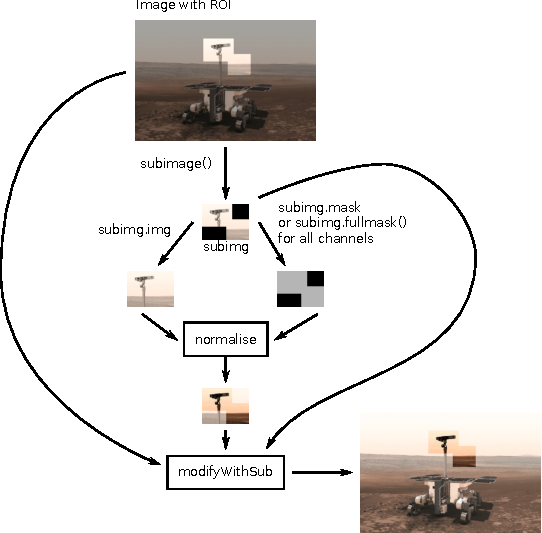
\includegraphics[width=5in]{norm.pdf}
\caption{The image processing in the norm node}
\label{norm.pdf}
\end{figure}
\clearpage
Finally, if the node was not enabled we set \texttt{node.img} (our output)
to be the input image:
\begin{lstlisting}
            else:
                node.img = img
\end{lstlisting}
and output the image to the node's zeroth (and only) output:
\begin{lstlisting}
        node.setOutput(0, node.img)
\end{lstlisting}


